% We are thrilled to announce the launch of the groundbreaking ByteBoost Cybertraining Program. ByteBoost is driven by the imperative to enhance researchers' proficiency and productivity when navigating cutting-edge, specialized computing technologies. We hope to empower researchers to make the best computing choices in the ever-changing landscape of computational technology. This initiative will focus on supporting researchers using the technologies of three NSF computing testbeds - Ookami, Neocortex and ACES.

% Program Objectives:
% Facilitate Seamless Research: Elevate the ease and productivity of researchers working with cutting-edge computing technology.
% Community Growth: Foster a well-informed community of computational researchers adept at handling the newest technologies and porting applications.
% Optimal Testbed Usage: Ensure the proper and efficient utilization of testbeds, a critical component in the recent surge of data-enabled science and engineering.
% Target Audience:
% Early career-researchers (graduate students, postdoctoral associates, and Assistant Professors) from all fields of computationally inclined research

% Submission Guidelines
% Submission must include the following
% CV (1 page) including the applicant's previous computing experiences, skills, and field of science
% Abstract (1 page) - Prospective participants are required to submit an abstract outlining the specific topic they intend to explore as a fundamental part of their application for consideration in this call for participation.
\noindent
\textbf{Foundations for Agent-based Evolution on Emerging HPC Accelerators.}
M.A. Moreno, \texttt{morenoma@umich.edu}

\section{Introduction}
Evolutionary processes underlie key questions in public health, medicine, and natural resources management.
In conjunction with benchtop experiments and observational studies, mathematical and computational models play a key role in understanding evolutionary processes underpinning critical problems like epidemiology, antibiotic resistance, cancer biology, and conservation biology.
Emerging High-Performance Computing (HPC) hardware like the Cerebras Wafer-Scale Engine (WSE) and Graphcore Intelligence Processing Unit (IPU) will enable detailed modeling of key cross-scale evolutionary phenomena, such as transitions of individuality (e.g., multicellularity) and evo-epidemiological tradeoffs between pathogens' within-host dynamics and between-host transmissibility \cite{goldsby2020major,schreiber2021evolutionary}.

\section{Objectives}

The proposed workshop project will explore foundational algorithms and supporting software (e.g., Cerebras Software Language [CSL], Poplar) necessary to harness emerging HPC hardware accelerators for agent-based evolution research.
Developed simulation will investigate how population structure and rare mutational events influence selective sweep frequency within very large populations.
Among other application areas, sweep dynamics are pivotal to understanding how new pathogen strains emerge and establish within host populations \cite{markov2023evolution}.

\section{Methods}

To succeed as a tool for scientific research, simulation must be sufficiently observable.
In the case of evolutionary simulation, phylogenetic history (i.e., ancestry trees) is key to assessing the mode and tempo of evolution.

\begin{wrapfigure}{R}{2in}
% \begin{minipage}{3in}
\vspace{-3ex}
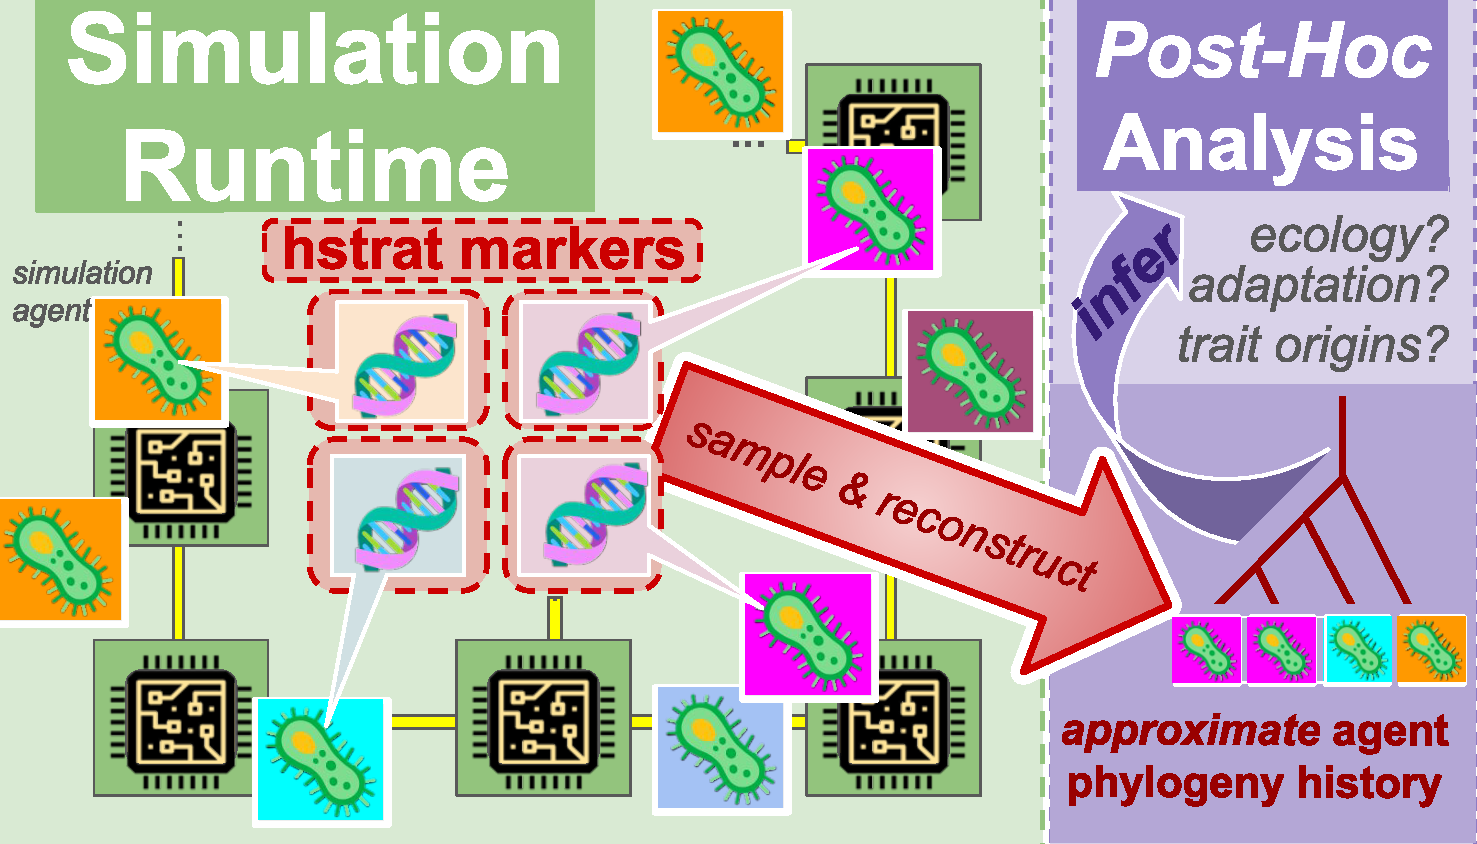
\includegraphics[width=2in]{img/runtime-posthoc-schematic.pdf}
% \end{minipage}%
% \begin{minipage}{2in}
\vspace{-5ex}
\caption{\footnotesize
Evolution simulation with reconstruction-based lineage analysis.}
\label{fig:runtime-posthoc-schematic}
\vspace{-2ex}
% \end{minipage}
\end{wrapfigure}


Proposed work builds on recently-introduced \textit{hereditary stratigraphy} (HStrat) methods designed to enable characterization evolutionary history in highly-distributed simulations \cite{moreno2022hstrat}.
These methods mark population members with a special annotation akin to noncoding DNA (as small as 96 bits), inherited by each consecutive generation.
After simulation ends, HStrat markers facilitate fast and accurate reconstruction of phylogenetic history.
This procedure, summarized in Figure \ref{fig:runtime-posthoc-schematic}, analogizes use of DNA sequence data to infer phylogenies of natural systems.
Unlike direct lineage tracking, HStrat methods scale gracefully to long-running multiprocess simulation \cite{moreno2024analysis}.

Simulation will use an island model to harness the processing power of focal HPC accelerators.
This approach instantiates separate agent subpopulations per processor, with agents occasionally migrated between subpopulations.
Global population structure results from rates of agent migration and the pattern of connectivity between islands.

A simple agent model suffices for proposed work, with agent traits abstracted to a floating point ``fitness'' value encoded directly in agent genomes.
Fitness landscape properties can be tuned through choice of mutation operator.
For instance, high probability deleterious outcomes would simulate a rugged landscape.

\section{Proposed Work}

Project work will focus on the Cererbras WSE platform.
Workshop activities will build on recent initial implementation of HStrat-enabled island model evolutionary simulation in CSL via the v1.0.0 Cerebras SDK.
Prototype code is available via GitHub at \url{hopth.ru/cl}.
Several engineering problems suited to workshop scope remain unresolved:
\begin{enumerate*}
\item \textbf{Agent migration between distant processing elements}.
Possible strategies include stochastic forwarding or more structured wavelet routing schemes.
This capability enables manipulation of population structure via island capability as an experimental variable.

\item \textbf{On-the-fly device-to-host genome sampling.}
Recording evolutionary intermediates over simulation runtime can help characterize evolutionary history, akin to a ``fossil record.''
\end{enumerate*}

\section{Broader Impacts}

I hope to amplify impact my own ByteBoost participation by sharing what I learn and create to empower others in my research community in two ways.
\begin{enumerate*}
\item \textbf{Software Products}: Availability of usable, extendable software significantly drives adoption and productivity of any new research platform.
I hope to strengthen community codebase by documenting, packaging, and sharing code developed during the course of the workshop.
Given the cutting-edge nascency of ByteBoost platforms, I anticipate great benefit learning best practices to organize, test, and distribute on-device kernel/on-host driver software components through discussion with other workshop participants.
\item \textbf{Knowledge Transfer}: I plan to report workshop highlights back to my peers at the BEACON Center and the Schmidt AI in Science Postdoc Program.
Both groups host rotating weekly meetings ideal for this purpose.
Within my own lab group, I will relay knowledge to undergraduate mentee Connor Yang currently working on CSL projects.
\end{enumerate*}

\section{Career Impact}

As an early-career researcher, ByteBoost provides a valuable opportunity to develop skills and professional connections to further my career goals to equip the digital evolution community to achieve radically scaled-up simulation.
I will roll workshop participation into a broader nascent research agenda.
In conjunction, I am presently developing an ACCESS Innovative Projects Proposal and recently entered a preproposal to the Dept. of Energy's EXPRESS 2024 FOA.
Ultimately, proposed work takes first steps in sustained leadership laying foundations for application of new accelerator technologies to agent-based modeling in digital evolution and beyond.

% will catalyze research.
% Progress on this front
% How to , to directly create modules during the workshop that can be shared.
% If there aren’t established protocols, the workshop environment would be a great place to discuss these issues.


% What is the structural relationship between individual-level phylogenies and species-level phylogenies?
% Do they respond in the same way to evolutionary conditions like selection pressure, ecology, and spatial structure?
